\subsubsection{Configuration Overhead}\label{cockpit::app:benchmark-configuration}

For the estimation of different \cockpit configuration overheads, we use almost
the same setting as described above, training for $512$ iterations and tracking
only every specified interval.

\subsubsection{Configuration Overhead on GPU Versus CPU}

\Cref{cockpit::fig:app_benchmark_configurations_cuda} and
\Cref{cockpit::fig:app_benchmark_configurations_cpu} show the configuration
overhead for four different \deepobs problems. The bottom left part of
\Cref{cockpit::fig:app_benchmark_configurations_cuda} corresponds to
\Cref{cockpit::fig:benchmark_heatmap}. In general, increased parallelism can be
exploited on a GPU, leading to smaller overheads in comparison to a CPU.

\cockpit can even scale to significantly larger problems, such as a \resnetfifty
on \imagenet-like data.
\Cref{cockpit::fig:app_benchmark_configurations_gpu_imagenet} shows the
computational overhead for different tracking intervals on such a large-scale
problem. Using the \textit{economy} configuration, we can achieve our
self-imposed goal of at most doubling the run time even when tracking every
fourth step. More extensive configurations (such as the \textit{full} set) would
indeed have almost prohibitively large costs associated. However, these costs
could be dramatically reduced when one decides to only inspect a part of the
network using \cockpit. Note, individual gradients are not properly defined when
using batch norm, therefore, we replaced these batch norm layers with identity
layers when using the \resnetfifty.

\captionsetup[subfigure]{justification=justified,singlelinecheck=false}

\begin{figure*}[t]
  \centering
  \begin{subfigure}[t]{0.35\linewidth}
    \centering
    \caption{\mnist \MNISTNET (GPU)}
    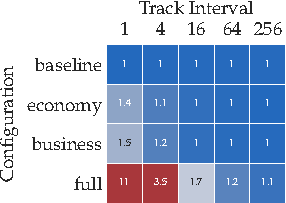
\includegraphics{../repos/cockpit-paper/fig/01_benchmark/output/fig_grid/benchmark_mnist_logreg_cuda_app_thesis-wide}
    \label{cockpit::fig:app_benchmark_configurations_cuda-mnist_logreg}
  \end{subfigure}
  \hspace{0.1\linewidth}
  \begin{subfigure}[t]{0.35\linewidth}
    \centering
    \caption{\mnist \mlp (GPU)}
    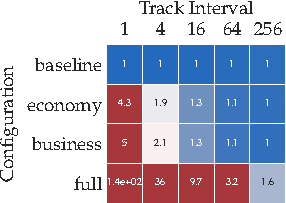
\includegraphics{../repos/cockpit-paper/fig/01_benchmark/output/fig_grid/benchmark_mnist_mlp_cuda_app_thesis-wide}
    \label{cockpit::fig:app_benchmark_configurations_cuda-mnist_mlp}
  \end{subfigure}
  \begin{subfigure}[t]{0.35\linewidth}
    \centering
    \caption{\cifarten \threecthreed (GPU)}
    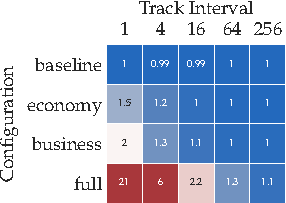
\includegraphics{../repos/cockpit-paper/fig/01_benchmark/output/fig_grid/benchmark_cifar10_3c3d_cuda_app_thesis-wide}
    \label{cockpit::fig:app_benchmark_configurations_cuda-cifar}
  \end{subfigure}
  \hspace{0.1\linewidth}
  \begin{subfigure}[t]{0.35\linewidth}
    \centering
    \caption{\fmnist \twoctwod (GPU)}
    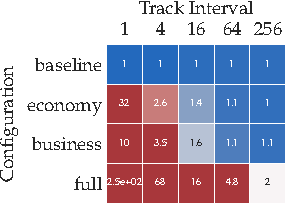
\includegraphics{../repos/cockpit-paper/fig/01_benchmark/output/fig_grid/benchmark_fmnist_2c2d_cuda_app_thesis-wide}
    \label{cockpit::fig:app_benchmark_configurations_cuda-fmnist}
  \end{subfigure}
  \caption{\textbf{Overhead of \cockpittitle configurations on GPU for four
      different problems with varying tracking interval.} Color bar is the same
    as in \autoref{cockpit::fig:benchmark}.}
  \label{cockpit::fig:app_benchmark_configurations_cuda}
\end{figure*}

\captionsetup[subfigure]{justification=centering, singlelinecheck=true}

%%% Local Variables:
%%% mode: latex
%%% TeX-master: "../../../thesis"
%%% End:


\captionsetup[subfigure]{justification=justified,singlelinecheck=false}

\begin{figure}[t]
	\centering
	\begin{subfigure}[t]{0.4\textwidth}
		\caption{\mnist Log.\,Reg.\,(CPU)}
		\includegraphics[width=\linewidth]{fig/01_benchmark/fig_grid/benchmark_mnist_logreg_cpu_app}
		\label{fig:app_benchmark_configurations_cpu-mnist_logreg}
	\end{subfigure}
	\hspace{0.06\textwidth}
	\begin{subfigure}[t]{0.4\textwidth}
		\caption{\mnist \mlp\,(CPU)}
		\includegraphics[width=\linewidth]{fig/01_benchmark/fig_grid/benchmark_mnist_mlp_cpu_app}
		\label{fig:app_benchmark_configurations_cpu-mnist_mlp}
		\vspace{0.25cm}
	\end{subfigure}
	\begin{subfigure}[t]{0.4\textwidth}
		\caption{\cifarten \threecthreed\,(CPU)}
		\includegraphics[width=\linewidth]{fig/01_benchmark/fig_grid/benchmark_cifar10_3c3d_cpu_app}
		\label{fig:app_benchmark_configurations_cpu-cifar}
	\end{subfigure}
	\hspace{0.06\textwidth}
	\begin{subfigure}[t]{0.4\textwidth}
		\caption{\fmnist \twoctwod\,(GPU)}
		\includegraphics[width=\linewidth]{fig/01_benchmark/fig_grid/benchmark_fmnist_2c2d_cpu_app}
		\label{fig:app_benchmark_configurations_cpu-fmnist}
	\end{subfigure}
	\caption{\textbf{Overhead of \cockpittitle configurations on CPU for four
			different problems with varying tracking interval.} Color bar is the same as in \autoref{fig:benchmark}.}
	\label{fig:app_benchmark_configurations_cpu}
\end{figure}

\captionsetup[subfigure]{justification=centering, singlelinecheck=true}

%%% Local Variables:
%%% mode: latex
%%% TeX-master: "../cockpit_paper"
%%% End:


\clearpage

\begin{figure}[t]
	\centering
	\includegraphics[width=0.59\linewidth]{fig/01_benchmark/fig_grid/benchmark_dummyimagenet_resnet50nobn_cuda_app}
	
	\caption{\textbf{Overhead of \cockpittitle configurations on GPU for \resnetfifty on
			\imagenet.} \cockpit's instruments scale efficiently even to very large problems
			(here: $1000$ classes, $(3, 224, 224)$-sized inputs, and a batch size of $64$.
			For individual gradients to be defined, we replaced the batch norm layers of the 
			\resnetfifty model with identities.) Color bar is the same as in \autoref{fig:benchmark}.}
	\label{fig:app_benchmark_configurations_gpu_imagenet}
\end{figure}


%%% Local Variables:
%%% mode: latex
%%% TeX-master: "../cockpit_paper"
%%% End:


%%% Local Variables:
%%% mode: latex
%%% TeX-master: "../thesis"
%%% End:
